%! Author = arqfa
%! Date = 2/7/2024

\documentclass[final,5p,times]{elsarticle}

%!Packages
%% The amssymb package provides various useful mathematical symbols
\usepackage{amssymb}
%% The amsthm package provides extended theorem environments
\usepackage{amsthm}
\usepackage{graphicx}
\usepackage{tabularx}
\usepackage{booktabs}
\usepackage{amsmath} % for equations
\usepackage{breakurl}
\usepackage{hyperref} % Ensure hyperlinks work properly


%% The lineno packages adds line numbers. Start line numbering with
%%\begin{linenumbers}, end it with \end{linenumbers}. Or switch it on
%% for the whole article with \linenumbers
\usepackage{lineno}
\modulolinenumbers[10]
\usepackage{enumitem}

%\usepackage{amsmath}

\usepackage{multirow}

\usepackage{caption}


% Document
\begin{document}

%!%!%Figures of 3D modeling and VR integration
%Figures "3d model vs real" and "Interior vs Exterior"
        \begin{table*}[htb]
            \centering
            \small
            \begin{tabular}{c}
                %Top cell with two figures
                \begin{minipage}{\textwidth}
                    \centering
                    % Left figure
                    %% Figure Real vs 3d Model
                    \begin{minipage}{0.49\textwidth}
                        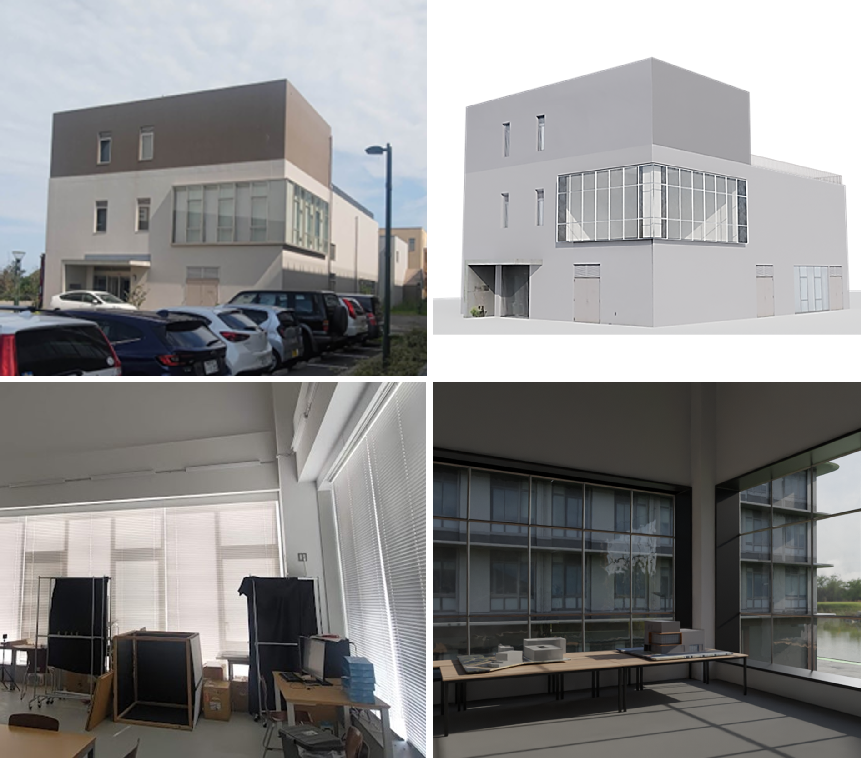
\includegraphics[width= \linewidth]{Images/Realvs3DmodelBlender}
                        \captionof{figure}{Real vs. 3D modeled building for the Facade Design Complexity Analysis experiment.}
                        \label{fig:RealVs3dModel}
                    \end{minipage}
                    \hfill % Spacing between the figures
                    % Right figure
                    %% FigureVR interior vs Exterior
                    \begin{minipage}{0.49\textwidth}
                        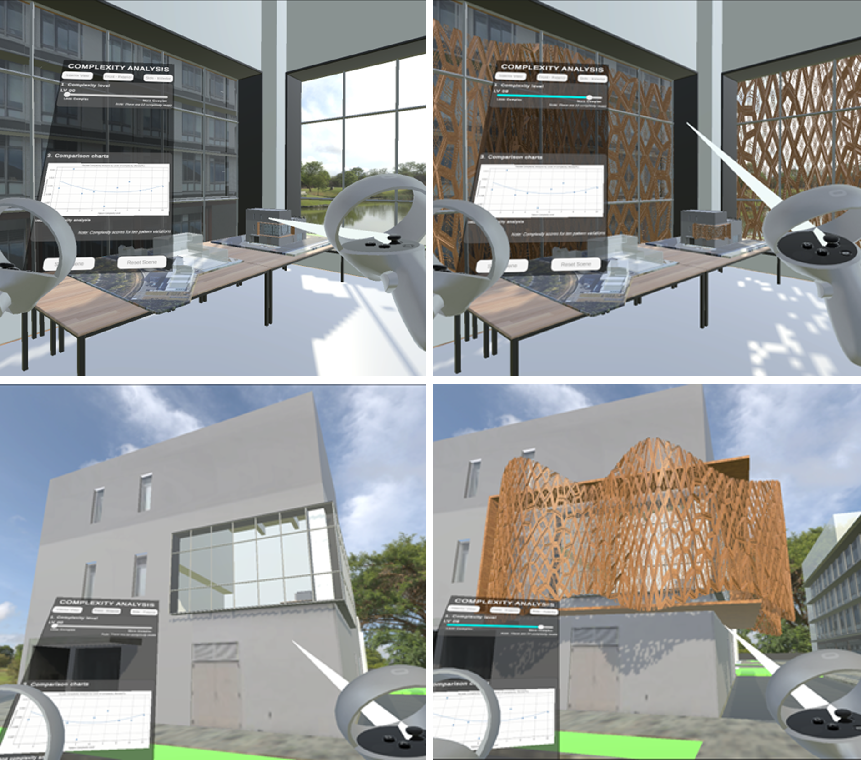
\includegraphics[width= \linewidth]{Images/VRInteriorExterior}
                        \captionof{figure}{Comparison side by side of the VR simulation of interior and exterior of existing laboratory building used for experiment (Left) and VR Simulation of facade variation (Right) used for complexity Analysis.}
                        \label{fig:VRInteriorExterior}
                    \end{minipage}
                \end{minipage}
            \end{tabular}
        \end{table*}


%!%Figures and table CICA
        %Flowchart CICA, Figure of Cica on historical buildings and renders, PI table. Table 1x3
        \begin{table*}[htb]
            \centering
            \small
            \begin{tabular}{c}
                %Top cell with one figure
                %Figure Computational Image Compexity Analysis (CICA) System flowchart
                \begin{minipage}{\textwidth}
                    \centering
                    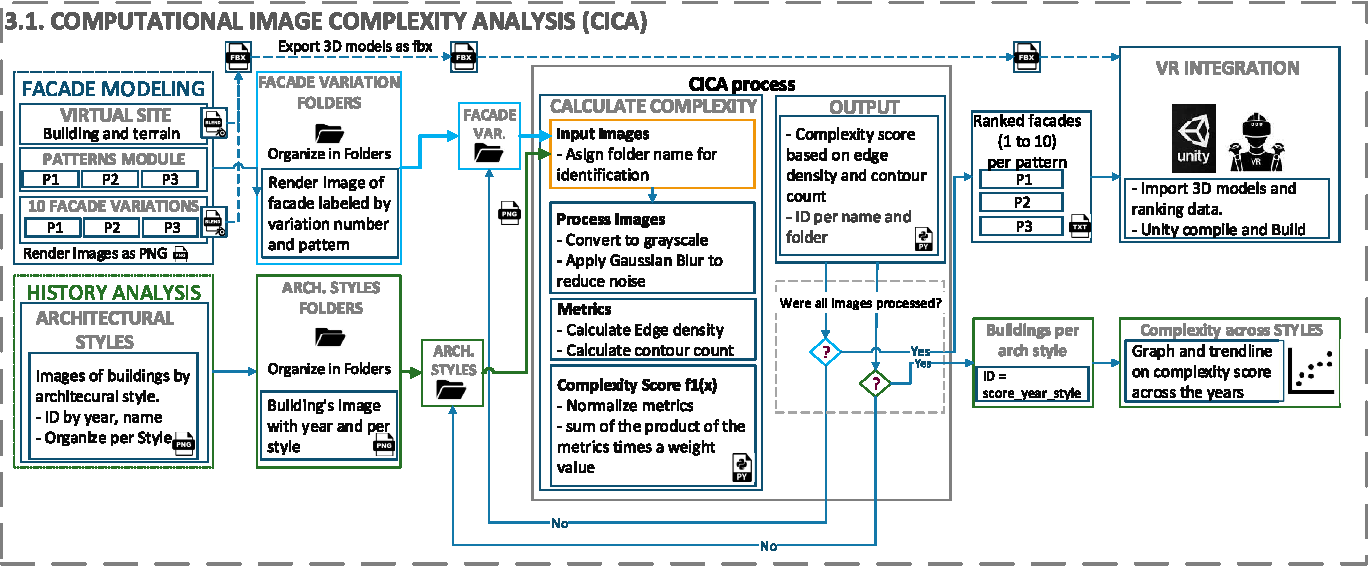
\includegraphics[width= \linewidth]{Images/ImageComplexityAnalysisFlowchart}
                    \caption{Flowchart illustrating the applications of Computational Image Complexity Analysis, including its role in analyzing complexity scores for historical architectural styles and ranking modeled facades for the VR Building Complexity System.}
                  \label{fig:ImageComplexityAnalysisFlowchart}
                \end{minipage}
                \\
                %Middle cell with two nested figures side by side
                %%%Figure CICA on historic buildings and renders. Table 1x2
                \begin{minipage}{\textwidth}
                    \centering
                    % Left figure
                    \begin{minipage}{0.49\textwidth}
                        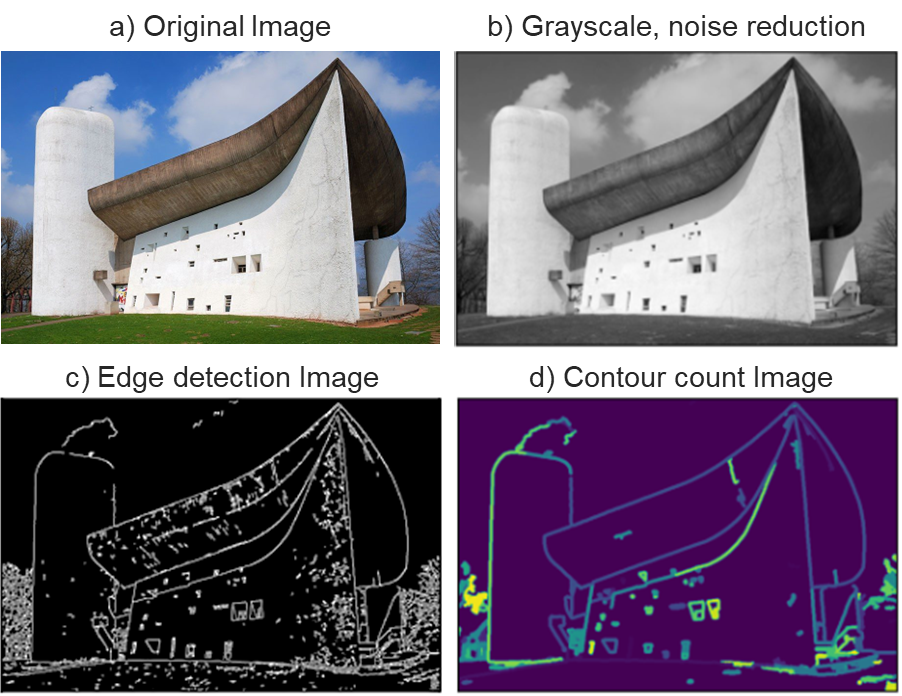
\includegraphics[width= \linewidth]{Images/CICAHistoryPlot}
                        \captionof{figure}{Edge Detection analysis of historic buildings demonstrating complexity assessment.}
                        \label{fig:ComplexityPlotHistory}
                    \end{minipage}
                    \hfill % Spacing between the figures
                    % Right figure
                    \begin{minipage}{0.49\textwidth}
                        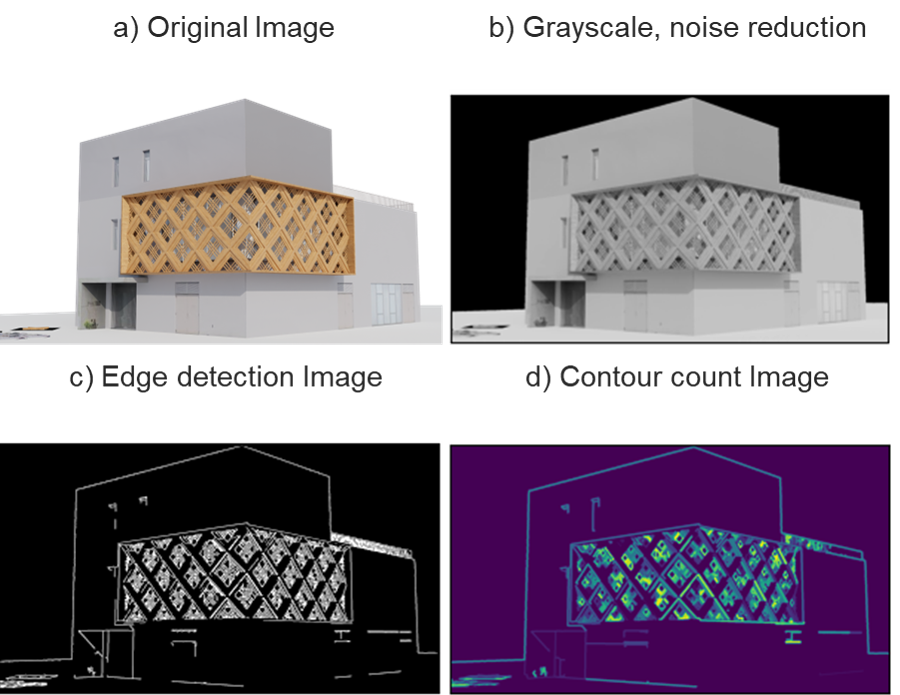
\includegraphics[width= \linewidth]{Images/CICARenderPlot}
                        \captionof{figure}{Complexity analysis of 3D-modeled facades for the VR experiment.}
                        \label{fig:ComplexityPlotRenderCICA}
                    \end{minipage}
                \end{minipage}
                \\
                %Bottom cell
                %Table: Performance Indicators
                \begin{minipage}{\textwidth}
                    \centering
                    \captionof{table}{Metrics and weights for the calculation of the `Complexity score'}
                    \label{tab:MetricsandWeights}
                    \begin{tabularx}{\textwidth}{p{3.5cm} p{1cm} X X p{1cm}}
                        \toprule
                        \textit{Complexity metric} &
                          \textit{N} &
                          \textit{Metric name/description} &
                          \textit{Quantitative   method} &
                          \textit{Weights} \\ \midrule
                        \textbf{Edge Density} &
                          1 &
                          Edge detection using Canny Edge Detection algorithm for highlighting the most relevant features of a building.
                            &
                          Measured by dividing the number of non-zero (edge) pixels in the edges image by the total number of pixels in the image.
                            &
                          8\\
                        \textbf{Contour count} &
                          2 &
                          Employs contour approximation algorithm for shape analysis to determine intricacy of edges.
                            &
                          Measure by counting the number of segments in an edge.
                            &
                          2\\ \bottomrule
                           &
                           &
                          \textbf{TOTAL} &
                          &
                          \textbf{10}\\ \bottomrule
                    \end{tabularx}
                \end{minipage}
                \\
                %Bottom cell with one figure
                \begin{minipage}{\textwidth}
                    \centering
                    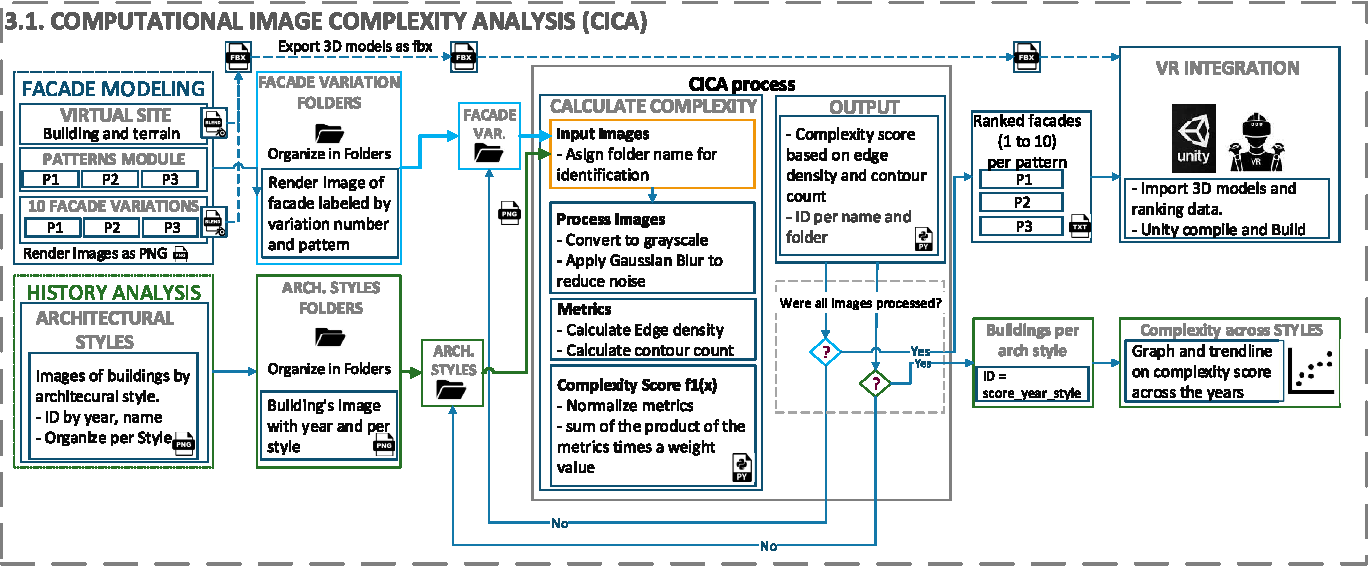
\includegraphics[width= \linewidth]{Images/ImageComplexityAnalysisFlowchart}
                    \caption{Flowchart illustrating the applications of Computational Image Complexity Analysis, including its role in analyzing complexity scores for historical architectural styles and ranking modeled facades for the VR Building Complexity System.}
                  \label{fig:ImageComplexityAnalysisFlowchart}
                \end{minipage}
            \end{tabular}
        \end{table*}


%!BackUp CICA
        %% Figure Computational Image Compexity Analysis (CICA) System flowchart
            \begin{figure*}[!htb]
                \centering
                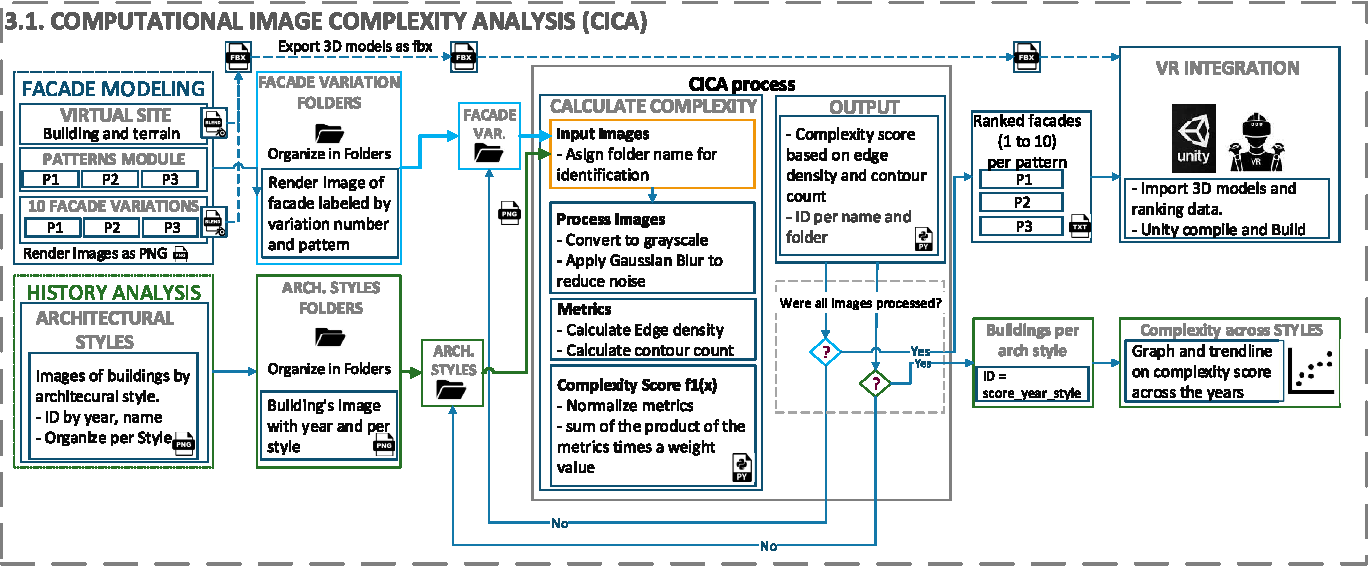
\includegraphics[width= \linewidth]{Images/ImageComplexityAnalysisFlowchart}~\caption{Flowchart illustrating the applications of Computational Image Complexity Analysis, including its role in analyzing complexity scores for historical architectural styles and ranking modeled facades for the VR Building Complexity System.}
                  \label{fig:ImageComplexityAnalysisFlowchart}
            \end{figure*}

            %%Figure CICA on historic buildings and renders. Table 1x2
            \begin{table*}[htb]
                \centering
                \small
                \begin{tabularx}{\textwidth}{X X}
                    \centering
                    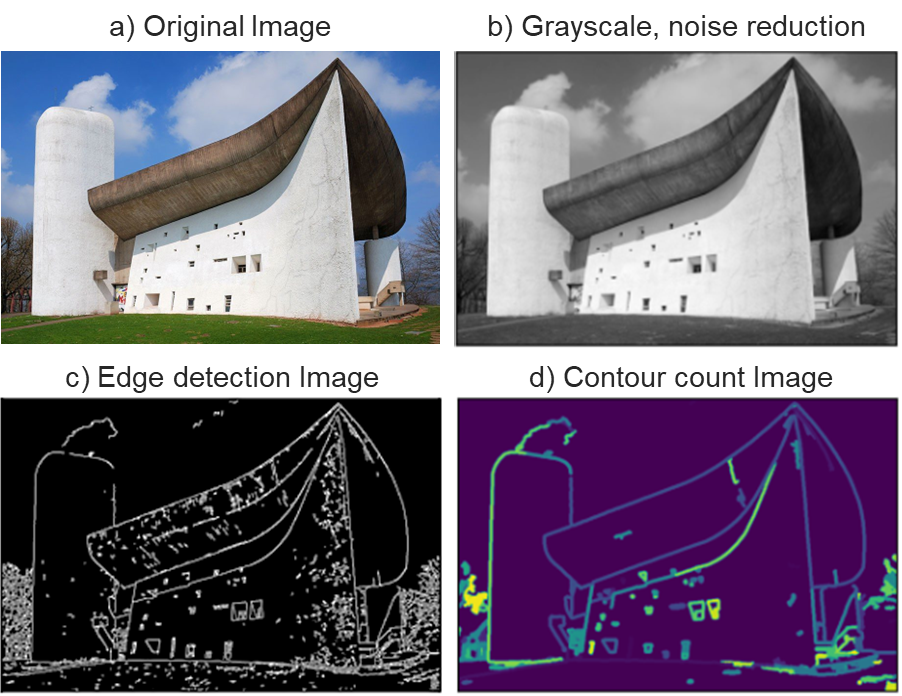
\includegraphics[width= \linewidth]{Images/CICAHistoryPlot}
                    \captionof{figure}{Edge Detection analysis of historic buildings demonstrating complexity assessment.}
                    \label{fig:ComplexityPlotHistory} &
                    \centering
                    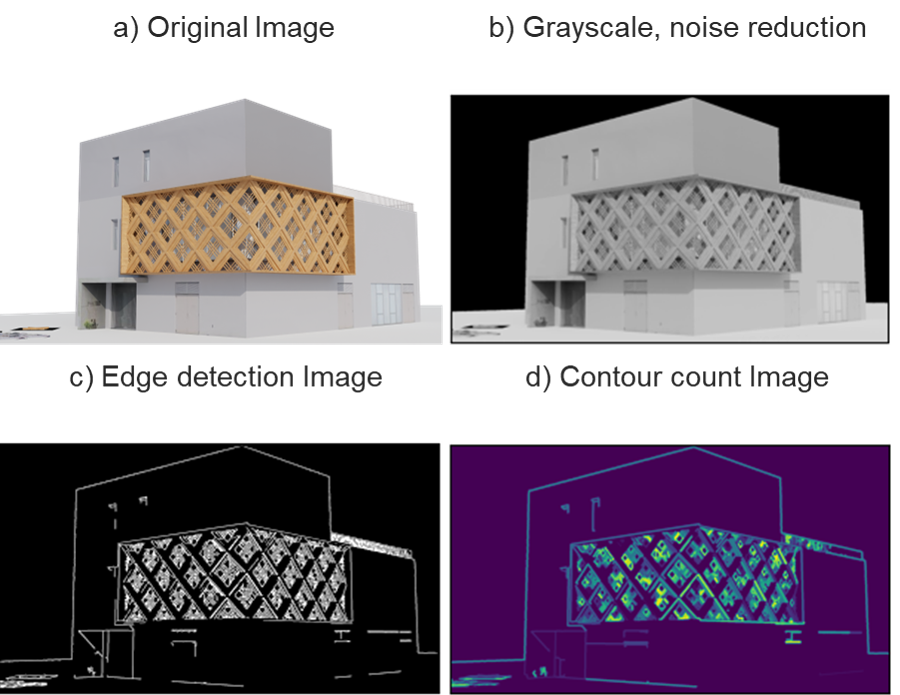
\includegraphics[width= \linewidth]{Images/CICARenderPlot}
                    \captionof{figure}{Complexity analysis of 3D-modeled facades for the VR experiment.}
                    \label{fig:ComplexityPlotRenderCICA}
                    \end{tabularx}
                \end{table*}

            %%Table: Performance Indicators
            \begin{table*}[htb]
                \centering
                \small
                \caption{Metrics and weights for the calculation of the `Complexity score'}
                \label{tab:MetricsandWeights}
                \begin{tabularx}{\textwidth}{p{3.5cm} p{1cm} X X p{1cm}}
                    \toprule
                    \textit{Complexity metric} &
                      \textit{N} &
                      \textit{Metric name/description} &
                      \textit{Quantitative   method} &
                      \textit{Weights} \\ \midrule
                    \textbf{Edge Density} &
                      1 &
                      Edge detection using Canny Edge Detection algorithm for highlighting the most relevant features of a building.
                        &
                      Measured by dividing the number of non-zero (edge) pixels in the edges image by the total number of pixels in the image.
                        &
                      8\\
                    \textbf{Contour count} &
                      2 &
                      Employs contour approximation algorithm for shape analysis to determine intricacy of edges.
                        &
                      Measure by counting the number of segments in an edge.
                        &
                      2\\ \bottomrule
                       &
                       &
                      \textbf{TOTAL} &
                      &
                      \textbf{10}\\ \bottomrule
                \end{tabularx}
            \end{table*}

%%%%%%%%%%%%%%%%%%%%
\end{document}